\documentclass[twoside]{article}
\usepackage{aistats2015}
\usepackage{graphicx}
\usepackage{pgfplots}
\usepackage{float}
\usepackage{subfig}
\usepackage{hyperref}
\usepackage{natbib}
\usepackage{amsmath}
\usepackage{amssymb}

\bibpunct{[}{]}{;}{n}{,}{,}

\newlength\figureheight \newlength\figurewidth % ?

\begin{document}

\twocolumn[
\aistatstitle{Learning to Control Kilobots with a Flashlight}
\aistatsauthor{Alexander Hendrich \And Daniel Kauth \And Gregor Gebhardt}
\aistatsaddress{TU Darmstadt \And TU Darmstadt \And TU Darmstadt}]

\begin{abstract}
The recently emerged kilobots provide lots of new applications for swarm
intelligence and collective behavior algorithms. By applying a light following
behavior called \emph{Phototaxis} to the kilobots, they provide an easy method
to move and control large quantities at the same time. By interacting with the
lightsource(s) (switching them on/off or moving a single light source) a human
can control a kilobot swarm to fulfill certain tasks, for example pushing an
object through a maze\cite{kilobotMaze}. In this project we want to learn to
control the light to achieve this behavior.
\end{abstract}

\section{INTRODUCTION}

Our task is to learn to push an object through a maze with a swarm of kilobots
by moving a single light source. Because this task is quite complex and
difficult to learn, we split it up into two separate problems with two separate
policies.

The first problem is to find an optimal path through the labyrinth. The policy
should return a movement direction for each possible object position. By
constantly following these movements, the object should reach the goal position
independent of its starting position.

Because we cannot directly control the object's movement we need a method to
interact with the light source, so that the kilobots push the object in the
desired direction. This will be the focus of the second problem. The policy
should return a new light position depending on the output of the first policy
(the desired movement direction of the object) and the relative position of the
kilobots towards the object.

\begin{figure}[!htb]
    \centering
    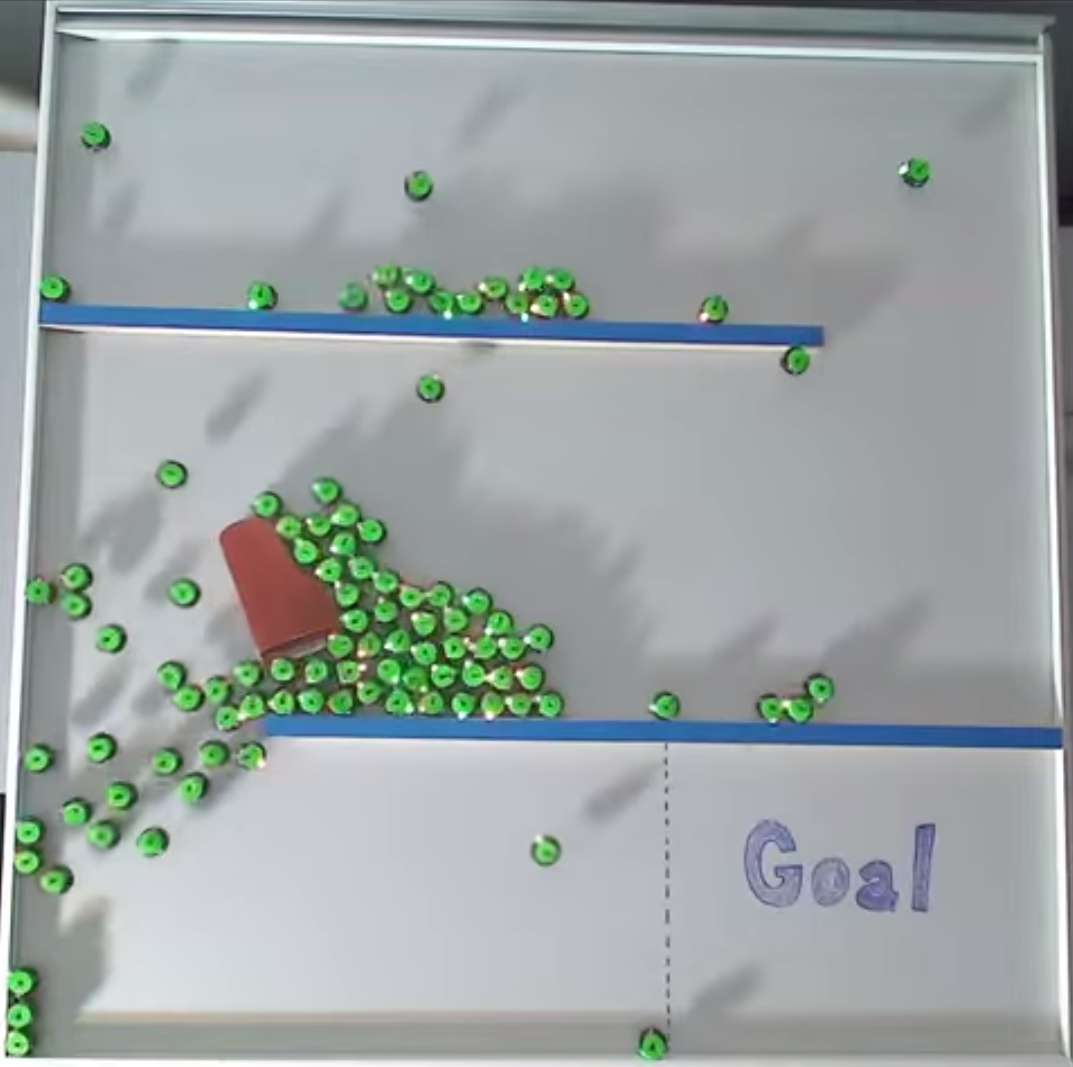
\includegraphics[width=0.8\linewidth]{figures/inspiration.png}
    \caption{Kilobots pushing a small object through a maze by human controlled
        light sources}
\end{figure}

\section{PRELIMINARIES}
In the following sections we introduce our used materials
(kilobots\cite{kilobot}) and methods (Actor Critic Relative Entropy Policy
Search)\cite{acreps}.

\subsection{Kilobots}
Kilobots\cite{kilobot} are open-source, low cost robots specially designed to
explore collective algorithms and decentralized cooperation. With previous
robots these methods could only be tested in a simulator or in small quantities
of robots because acquiring and controlling hundreds or even thousands of them
is very cost-intensive, time consuming and complex. To eliminate this issue
Harvard University developed Kilobots. Each robot is made with only 14\$ worth
of parts and large collectives can easily be controlled by a single user.

The low cost however results in limited capabilities of each individual robot.
For example, the kilobot doesn't use complex steering or wheels for locomotion.
Instead it stands on three solid legs and moves by activating two small
vibrating motors placed on each side of the kilobot. This form of movement only
allows for very low movement speeds of up to 1cm per second and can only be
performed on special surfaces (e.g. glass).

To communicate with each other, each kilobot has an infrared transmitter and
receiver on the bottom. Messages are passed by emitting infrared light onto the
reflecting glass and can be received by another kilobot up to 7-10cm away
(radius of each kilobot is 3.3cm). By measuring the received signal strength,
the kilobots are capable of estimating their distances to each other.

The kilobot also possesses an ambient light sensor to determine the light
intensity at its current location. Depending on the current and previously
measured light intensity the robot alternates between left and right turns to
move towards the light source. This behavior is called \emph{Phototaxis} and is
used to control a whole swarm of robots at once. While performing left or right
turns the robot only activates one of its two motors and the robot doesn't move
in a straight line, which further reduces its movement speed.

\begin{figure}[!htb]
    \centering
    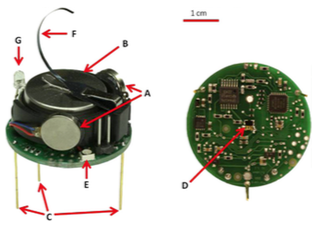
\includegraphics[width=0.9\linewidth]{figures/kilobot.png}
    \caption{Isometric (left) and bottom (right) views of a Kilobot. Some key
        features are: (A) vibration motors, (B) lithium-ion battery, (C) rigid
        supporting legs, (D) infrared transmitter/receiver, (E) three-color
        (RGB) LED, (F) charging tab, and (G) ambient light sensor. Note the 1 cm
        line for scale.\cite{kilobot}}
\end{figure}

\subsection{Actor Critic Relative Entropy Policy Search}
\emph{Actor critic relative entropy policy search} (AC-REPS) as introduced by
\cite{acreps} is a method for policy improvement based on \emph{relative entropy
policy search} (REPS) \cite{reps} which allows for model-free learning with
non-parametric continuous policies and random exploration. It consists of the
following three steps:

\subsubsection{Estimating the Q-Function}
\label{sec:estimateq}

During the simulation we generate sample in the form $(s_i, a_i, r_i, s'_i)$,
where we start in state $s_i$, take action $a_i$ to get to state $s'_i$ and
get reward $r_i$. We also define a feature-based Q-function as $Q(s, a) =
\phi(s,a)^T \theta$ with feature function $\phi(s,a)$ and parameter vector
$\theta$. Details of our state and action representations and rewards and
features we used are discussed in section \ref{sec:objpolicy}.

To estimate $\theta$ we use \emph{Least-squares temporal difference
learning} (LSTD) with $L_{22}-Regularization$\cite{lstdRegularization} as
follows:

With $n$ being the number of sample and $k$ being the number of features
we define the two feature matrices $\Phi$ and $\Phi'$ (size $n\times k$)
$$
\Phi = \left(
\begin{array}{c}
    \phi(s_1,a_1)^T \\
    \phi(s_2,a_2)^T \\
    \dots \\
    \phi(s_n,a_n^T)
\end{array} \right), \;
\Phi' = \left(
\begin{array}{c}
    \mathbf{E}_{\pi(a_1'|s_1')} [\phi(s_1', a_1') | s_1']^T \\
    \mathbf{E}_{\pi(a_2'|s_2')} [\phi(s_2', a_2') | s_2']^T \\
    \dots \\
    \mathbf{E}_{\pi(a_n'|s_n')} [\phi(s_n', a_n') | s_n']^T \\
\end{array} \right)
$$
and the reward vector
$$
R = \left(
\begin{array}{c}
    r(s_1) \\
    r(s_2) \\
    \dots \\
    r(s_n)
\end{array} \right).
$$
For $\Phi'$ we estimate the expected value
$$
\mathbf{E}_{\pi(a_i'|s_i')} [\phi(s_i', a_i') | s_i']
$$
by taking the average over $m$ samples $a_i' \sim \pi(a_i'|s_i')$, where $\pi$
is our current policy.

Using the derivations of \cite{lspi} and \cite{lstdRegularization} we can easily
compute $\theta$ as
$$
\theta = (X^TX+\beta'I)^{-1}X^Ty
$$
with
$$X = C(A+\beta I) \qquad y=Cb$$
$$A = \Phi^T(\phi-\gamma \Phi') \qquad b=\Phi^T R$$
$$C = \Phi(\Phi^T\Phi+\beta I)^{-1},$$
where $\beta$ and $\beta'$ are regularization parameters for the projection and
fixed-point step which make the estimation numerically more stable and improve
noise tolerance.

\subsubsection{Actor Critic REPS}
\label{sec:reps}

In this step we find a new policy $\pi'$ which optimizes the expected Q-value
as given by our estimated Q-function, but has a limited Kullback-Leibner (KL)
distance to the old policy $\pi$.

To achieve this we optimize over the joint state action distribution
$p(s,a) = p(s) \pi'(s, a)$ and require that the estimated state distribution
$p(s)$ is the same as in the given state sample distribution $\mu(s)$.
This is implemented by matching feature averages of $p(s)$ and $\mu(s)$ and
leads to the following optimization problem:
\begin{align*}
    & \max_p \int p(s, a)Q(s, a)\:ds\:da\:, \\
    & \text{s.t. } \text{KL}(p(s, a) || \mu(s)\pi(a|s)) \leq \epsilon,\\
    & \int p(s)\phi(s)\:ds = \hat{\phi}, \int p(s, a)\:ds\:da = 1,
\end{align*}
where $\hat{\phi} = \int p(s) \phi(s)\:ds$ is the average feature vector of all
state samples, $\phi(s)$ is another feature function and $\epsilon$ is the
maximum allowed distance between the old and new policies.

This problem can be solved using Lagrangian multipliers and has the solution
$$
p(s)\pi'(a|s) \propto \mu(s) \pi(a|s) \exp\left(\frac{Q(s,a) - V(s)}{\eta}\right),
$$
where $V(s) = v^T \phi(s)$ and $\eta$ and $v$ are Lagrangian multipliers which
can be obtained by minimizing the dual function on the samples using standard
gradient methods.

\subsubsection{Obtaining a new Policy}
\label{sec:gp}

The previous step only gives us desired probabilities
$p(s_i, a_i) = p(s_i) \pi'(a_i|s_i)$ for our samples so in this step we need
to generalize these by fitting a new policy $\bar{\pi}$.

This is done by minimizing the KL divergence between $\pi'$ and our new policy
$\bar{\pi}$ which is equivalent to computing a weighted maximum likelihood
estimate with sample weights
$$ w_i = \exp\left(\frac{Q(s_i, a_i) - V(s_i)}{\eta}\right). $$

In this paper we use a weighted Gaussian Process (GP) to obtain our new policy
$\bar{\pi}$ by estimating action $a_i$ for state $s_i$ with weight $w_i$. We
also use the sparse version of the GP as introduced in \cite{sparsegp} to reduce
computation time.

This choice of weights will reproduce actions which lead to a higher reward with
higher probability but will also choose suboptimal actions with some
probability. This behavior occurs because our new policy can not be too far away
in terms of KL divergence from the old policy and we start with a random policy.
This achieves a trade-off between exploration and exploitation.

\section{LEARNING PROCESS}

Our learning process is implemented in Python and uses a simple kilobot
simulator (see \ref{sec:simulator}) written by us to generate samples.

\subsection{Maze Solving Policy}
This policy tells us where the object should move given the current object
position and solves a maze (\autoref{fig:simulator}) in this way.

Because this policy is relatively easy to learn and there are specialized path
planning algorithms like $A^*$ which can easily compute an optimal path through
any maze we did not learn this policy and instead focused on the second one,
which is much more interesting. Therefore we manually specified this policy by
providing a number of waypoints the object should pass and give the next
waypoint as the target position. Once we reach a waypoint we move one to next
one.

In our experiments this simple policy is sufficient to move different objects
through a simple maze using our object movement policy. For this reason we will
only discuss the object movement policy in the following sections.

\subsection{Simulator}
\label{sec:simulator}

\newcommand\nkb{n_\mathit{kb}}
\newcommand\nep{n_\mathit{ep}}
\newcommand\nst{n_\mathit{st}}

We did not use a general purpose robot simulator like V-REP\cite{vrep}, because
it would take much longer than necessary to generate samples as the kilobots are
simulated more accurately than needed for our task. Instead we wrote our own
simple kilobot simulator (\autoref{fig:simulator}) in Python based on the 2D
physics engine pybox2d\cite{pybox2d}. This allows us to simulate collisions
between kilobots and other kilobots, the object and walls.

When requesting new samples from the simulator we specify the current policy
$\pi$ which will be used to generate these samples as well as the sampling
parameters such as the shape of the object, the number of kilobots $\nkb$, the
number of episodes $\nep$ and the number of steps per episode $\nst$.

Given these parameters the simulator first generates $\nep$ kilobot start
positions $\mathit{start}_i$ equally spaced in a circle of radius $1.5 \cdot r$
around the object which starts in the middle of the screen, where $r$ is the
radius or half-width of the object depending on the its shape. Then for
$i \in \{1, \dots, \nep\}$ we do the following:

The object's position is reset to the middle of the screen and its angle is set
to 0. After that the light position is set to $\mathit{start}_i$ and the
position of the $\nkb$ kilobots is set to $\mathit{start}_i + \mathit{off}_j$,
where $\mathit{off}_j$ is a small individual offset for kilobot number $j$.
Then $\nst$ time steps are simulated where in each one an action $a_k$ is chosen
for the current state $s_k$ according to $\pi$ and applied by adding $a_k$ to
the current light position. Next the kilobots move directly toward the light for
a short amount time (1 second for all of our simulations) and lastly we record
the current state as $s_k'$, compute the reward $r_k$ and save the tuple $(s_k,
a_k, r_k, s_k')$ as a sample. We also restrict the magnitude of the light and
kilobot movements to get a more realistic simulation.

The simulator can also be used to simulate the kilobots pushing an object
through a maze. In this mode we do not record any samples. Instead we move the
light according to our object movement policy which gets a target position from
our maze solving policy. The policies are combined in the following way:

As we will discuss in \ref{sec:objpolicy} our object movement policy learns
how to move the light to push the object to the right given the current light
and kilobot positions relative to the object's position. The maze solving policy
now gives us a target position $t$ from which we compute the target direction as
$d = t - o$ where $o$ is the current object position. We now compute the angle
$\alpha$ between $d$ and $(1, 0)$ (the vector pointing to the right) and rotate
the state around $\alpha$. Then we use the object movement policy to get an
action for our rotated state which we rotate by $-\alpha$ to get the final
action which we apply just as in the sample generation case.

\begin{figure}[!htb]
    \centering
    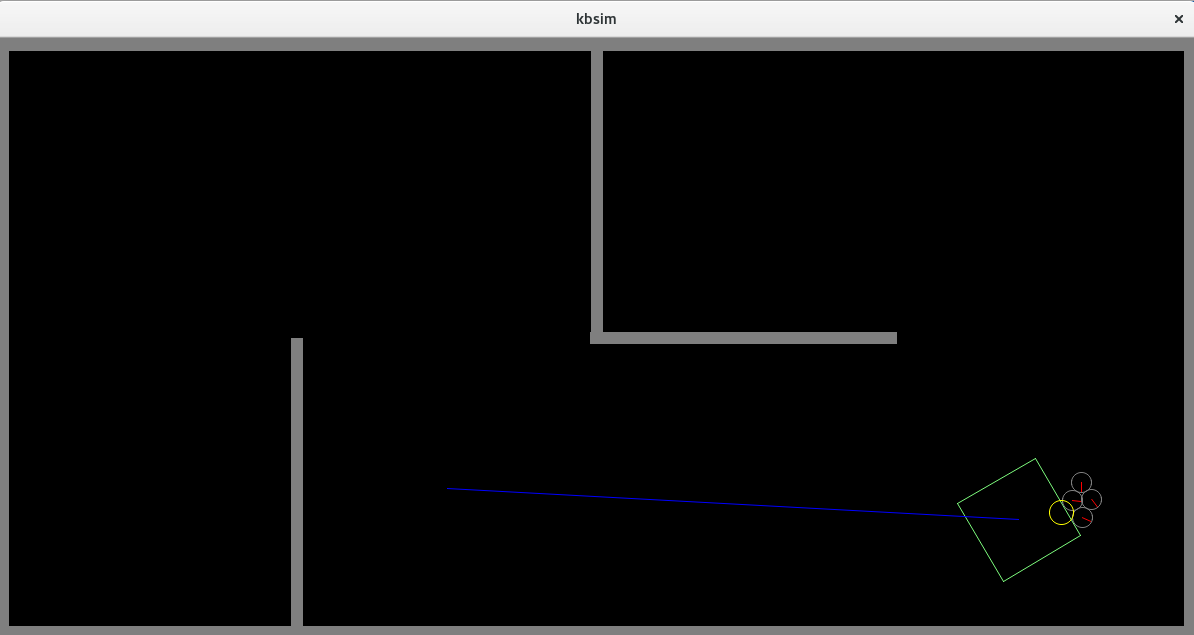
\includegraphics[width=0.9\linewidth]{figures/simulator_maze.png}
    \caption{4 kilobots pushing an object through a maze in the simulator.}
    \label{fig:simulator}
\end{figure}

\subsection{Object Movement Policy}
\label{sec:objpolicy}

For this policy we decided to only learn how to push the object to the right
instead of an arbitrary direction. This simplifies and speeds up the learning
process because we need to generate fewer samples and can represent our policy
using a smaller state subset for the sparse GP and therefore can compute the
policy update much faster. As discussed in the last paragraph of the previous
section we can still use this policy to push the object in an arbitrary
direction by rotating the state and action appropriately.

\subsubsection{On-Policy Learning}

To learn the object movement policy we use on-policy learning. During this
process we have matrices $S_k, A_k, R_k, S'_k$ with $n$ rows holding the $n$
current samples which are initially empty and a current policy $\pi_k$. Our
first policy $\pi_0$ predicts random actions $(a_x, a_y)$, where both $a_x$ and
$a_y$ are sampled uniformly from $[-0.015, 0.015]$ (1.5 cm).

In each iteration we use the current policy $\pi_k$ to generate $m$ samples
$(s_i, a_i, r_i, s'_i)$ and add them to the current samples giving matrices
$S_{k+1}, A_{k+1}, R_{k+1}, S'_{k+1}$ holding $n + m$ samples. To keep the
computation tractable we then randomly choose $10000$ of the $n + m$ samples
and replace the current sample matrices by matrices filled with the chosen
$10000$ samples (if $(n + m) < 10000$ nothing changes).

Next we estimate the Q-function as described in \ref{sec:estimateq},
compute a sample weighting as in \ref{sec:reps} and lastly fit a new sparse
GP as discussed in \ref{sec:gp}, which then becomes our new policy $\pi_{k+1}$.

We repeat these steps a fixed number of times and manually inspect the learned
policy. If it is not satisfactory (it can not solve the maze) we continue the
learning process.

\subsubsection{States and Actions}

With $n$ kilobots our state tuple is
$$s = (l_x, l_y, k_{1x}, k_{1y}, \dots, k_{nx}, k_{ny}), $$
where $(l_x, l_y)$ is the light position and $(k_{ix}, k_{iy})$ is the position
of the $i-th$ kilobot. All positions are relative to the object's center
position.

Our action tuple is
$$a = (a_x, a_y),$$
which is the direction the light should move in.

\subsubsection{Rewards}

Our reward is given by
$$ r = (c_x - p_x) - 0.5 \cdot |c_y - p_y|, $$
where $(c_x, c_y)$ is the object's current position and $(p_x, p_y)$ is the
object's position from the last time step. Therefore we reward movement to the
right and punish movement to the left and any movement in $y$ direction.

\subsubsection{Features and Kernels}

For our learning process we need a feature function $\phi(s, a)$ over
state-action pairs to represent our Q-function, a feature function $\phi(s)$
over states for REPS and a kernel function $K(s_1, s_2)$ between states for the
GP.

The feature functions are implemented in terms of kernel functions by
choosing a random subset of $N$ samples $(s_i, a_i)$ in each iteration and
computing the feature vectors for a given state $s$ and action $a$ as:
$$
\phi(s, a) = \left(
\begin{array}{c}
    K'((s_1, a_1), (s, a)) \\
    K'((s_2, a_2), (s, a)) \\
    \dots \\
    K'((s_N, a_N), (s, a))
\end{array} \right),
$$
$$
\phi(s) = \left(
\begin{array}{c}
    K(s_1, s) \\
    K(s_2, s) \\
    \dots \\
    K(s_N, s)
\end{array} \right),
$$
where $K'$ is a kernel function similar to $K$ which compares state-action
pairs. For our experiments we used $N = 200$.

Let $s$ be a state with $n$ kilobots with positions $(k_{ix}, k_{iy})$
and $s'$ be a state with $m$ kilobots with positions $(k'_{jx}, k'_{jy})$ and
let $a$ and $a'$ be the corresponding actions.
We define $K(s, s')$ and $K'((s, a), (s', a'))$ as follows:

First we compute the distance between the two kilobot configurations as
\begin{align*}
d_{kb} =
  \frac{1}{n^2} &\sum_{i,j \in \{1,\dots,n\}}
    \bar{K}((k_{ix}, k_{iy}), (k_{jx}, k_{jy})) \\
- \frac{2}{n \cdot m} &\sum_{\substack{i \in \{1,\dots,n\}\\j \in \{1,\dots,m\}}}
    \bar{K}((k_{ix}, k_{iy}), (k'_{jx}, k'_{jy})) \\
+ \frac{1}{m^2} &\sum_{i,j \in \{1,\dots,m\}}
    \bar{K}((k'_{ix}, k'_{iy}), (k'_{jx}, k'_{jy})),
\end{align*}
where $\bar{K}$ is a 2 dimensional squared exponential kernel with
$$
\bar{K}(k_1, k_2) =
    \exp \left(-0.5 (k_1 - k_2)^T
    \mathrm{diag}\left(\frac{1}{\sigma_{kb}^2}\right) (k_1 - k_2)\right)
$$
and $\sigma_{kb} \in \mathbb{R}^2$ is the bandwidth for the kilobot dimensions.
This allows us to compare states with different numbers of kilobots and the
computed distance is independent of the order of the kilobot positions in the
state vectors.

After that we compute the distance for the other dimensions (light positions for
$K$ and light positions and actions for $K'$) as
$$
d_{other} = (x_1 - x_2)^T \mathrm{diag}\left(\frac{1}{\sigma_{other}^2}\right) (x_1 - x_2),
$$
where $x_1$ and $x_2$ are vectors holding the values for all non-kilobot
dimensions and $\sigma_{other}$ is the non-kilobot bandwidth.

We combine these distances to get the kernel value
$$
\exp(-0.5 (w \cdot d_{other} + (1 - w) \cdot d_{kb})),
$$
where $w \in [0,1]$ weighs the importance of the non-kilobot dimensions.

In our experiments we used $w = 0.5$ and recomputed $\sigma_{kb}$ and
$\sigma_{other}$ in each iteration as the square root of the median of the
squared distances between all sample values for each dimension separately. We
also scaled the bandwidths uniformly in each dimension by some manually
specified factors.

\section{RESULTS}

For our final evaluation we made 20 runs of our learning process with 15
iterations each generating $25 \cdot 100 = 2500$ samples per iteration. Using
an Haswell Quad Core with 3.4GHz per core each iteration took about 3 minutes,
so the total run-time for each policy was about 45 minutes.

The policies start of only being able to push the object when the kilobots start
to the left of the object. After about 5 iterations they can also handle kilobot
starting positions above and below the object by first moving the kilobots
around to the left side of the object and then pushing the object from the left
side. After further iterations the policies are able to push the object to the
right even if the kilobots start above and to the right of the object (see
\autoref{fig:policyEvolution}). With even more iterations the kilobot starting
positions from which the object can be pushed tend to extend even further, but
this improvement is inconsistent and the policies may even get worse again.
Therefore we manually inspected the policies at each iteration and chose a good
policy (which is typically found in the first about 15 iterations) for solving
the maze.

\begin{figure*}[!htb]
	\centering
	\subfloat[Policy after 1 iteration]{
        \def\svgwidth{0.45\textwidth}
        \input{figures/policy_1.pdf_tex}
    }
    \hfill
	\subfloat[Policy after 5 iterations]{
        \def\svgwidth{0.45\textwidth}
        \input{figures/policy_5.pdf_tex}
    }
    \hfill
	\subfloat[Policy after 10 iterations]{
        \def\svgwidth{0.45\textwidth}
        \input{figures/policy_10.pdf_tex}
    }
    \hfill
	\subfloat[Policy after 15 iterations]{
        \def\svgwidth{0.45\textwidth}
        \input{figures/policy_15.pdf_tex}
    }
    \hfill
	\caption[foo]{Evolution of the learned policy}
	\label{fig:policyEvolution}
\end{figure*}

The value function (after 8 iterations) also shows that kilobot positions left
of the object are preferable to positions to the right. Further it increases
when moving around the object from the right to the left (see \autoref{fig:value}).

\begin{figure}[!htb]
	\centering
    \def\svgwidth{\columnwidth}
    \input{figures/value.pdf_tex}
    \caption{Learned value function after 8 iterations. The object (not shown
             here) is at the middle of the image.}
	\label{fig:value}
\end{figure}

With improving policies the object can be pushed to the right from a larger
number of kilobot starting positions. Additionally the object can be pushed
faster and with less vertical movement. Therefore the reward tends to increase
(see \autoref{fig:meanReward}).

\begin{figure}[!htb]
    \centering
    \resizebox{\linewidth}{!}{% Title: glps_renderer figure
% Creator: GL2PS 1.3.9, (C) 1999-2015 C. Geuzaine
% For: Octave
% CreationDate: Wed Mar  9 16:27:33 2016
\setlength{\unitlength}{1pt}
\begin{picture}(0,0)
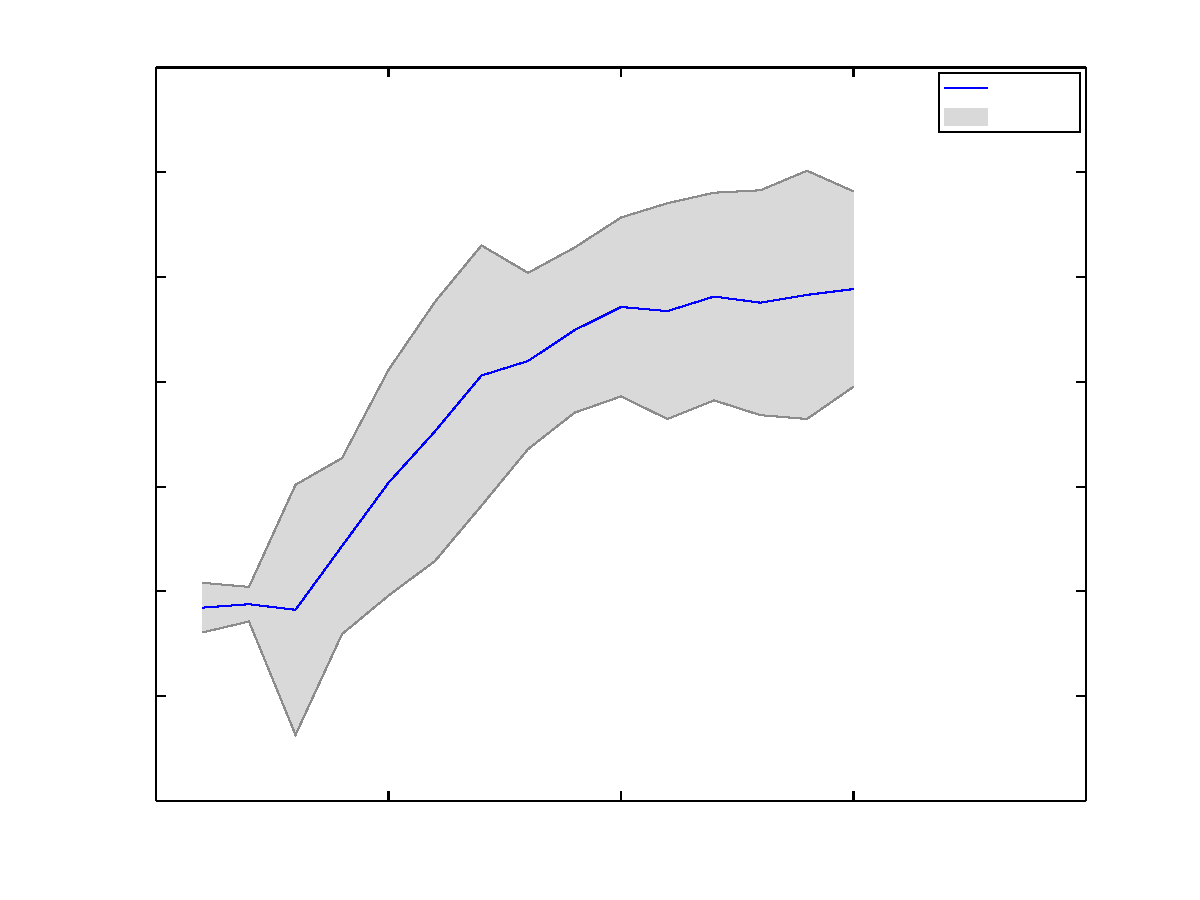
\includegraphics{figures/reward-inc}
\end{picture}%
\begin{picture}(576,432)(0,0)
\fontsize{10}{0}
\selectfont\put(74.8799,42.519){\makebox(0,0)[t]{\textcolor[rgb]{0,0,0}{{0}}}}
\fontsize{10}{0}
\selectfont\put(186.48,42.519){\makebox(0,0)[t]{\textcolor[rgb]{0,0,0}{{5}}}}
\fontsize{10}{0}
\selectfont\put(298.08,42.519){\makebox(0,0)[t]{\textcolor[rgb]{0,0,0}{{10}}}}
\fontsize{10}{0}
\selectfont\put(409.68,42.519){\makebox(0,0)[t]{\textcolor[rgb]{0,0,0}{{15}}}}
\fontsize{10}{0}
\selectfont\put(521.28,42.519){\makebox(0,0)[t]{\textcolor[rgb]{0,0,0}{{20}}}}
\fontsize{10}{0}
\selectfont\put(69.8755,47.52){\makebox(0,0)[r]{\textcolor[rgb]{0,0,0}{{-4}}}}
\fontsize{10}{0}
\selectfont\put(69.8755,97.8169){\makebox(0,0)[r]{\textcolor[rgb]{0,0,0}{{-2}}}}
\fontsize{10}{0}
\selectfont\put(69.8755,148.114){\makebox(0,0)[r]{\textcolor[rgb]{0,0,0}{{0}}}}
\fontsize{10}{0}
\selectfont\put(69.8755,198.412){\makebox(0,0)[r]{\textcolor[rgb]{0,0,0}{{2}}}}
\fontsize{10}{0}
\selectfont\put(69.8755,248.708){\makebox(0,0)[r]{\textcolor[rgb]{0,0,0}{{4}}}}
\fontsize{10}{0}
\selectfont\put(69.8755,299.006){\makebox(0,0)[r]{\textcolor[rgb]{0,0,0}{{6}}}}
\fontsize{10}{0}
\selectfont\put(69.8755,349.303){\makebox(0,0)[r]{\textcolor[rgb]{0,0,0}{{8}}}}
\fontsize{10}{0}
\selectfont\put(69.8755,399.6){\makebox(0,0)[r]{\textcolor[rgb]{0,0,0}{{10}}}}
\fontsize{10}{0}
\selectfont\put(298.08,31.519){\makebox(0,0)[t]{\textcolor[rgb]{0,0,0}{{iteration}}}}
\fontsize{10}{0}
\selectfont\put(53.8755,223.56){\rotatebox{90}{\makebox(0,0)[b]{\textcolor[rgb]{0,0,0}{{reward}}}}}
\fontsize{10}{0}
\selectfont\put(476.711,389.831){\makebox(0,0)[l]{\textcolor[rgb]{0,0,0}{{mean}}}}
\fontsize{10}{0}
\selectfont\put(476.711,375.774){\makebox(0,0)[l]{\textcolor[rgb]{0,0,0}{{$2 \sigma$}}}}
\end{picture}
}
    \caption{Total reward for each iteration averaged over 20 runs. The shaded
             area shows twice the standard deviation.}
    \label{fig:meanReward}
\end{figure}

We made the policy plots by getting the mean action for states distributed on a
grid and plotting it as an arrow indicating the direction the light should move
in. For this we set the relative light positions to evenly spaced values between
$-0.25$ and $0.25$ for the $x-$ and $y-$dimensions and set the position for all
kilobots to coincide with the light position.

To compute the Value-function we use the same states and uniformly sample a
number of actions at random for each state. Then we compute the Q-values for all
state-action pairs and average them for each state.

To evaluate our policies we used our simulator to push the object through the
maze as described in \ref{sec:simulator}. We found that our learned policies are
sufficient to achieve this task and are even able to move the object when the
kilobots are (almost) completely on the wrong side of the object, which requires
moving them around the object. Moreover we can transfer our policy to more or
less kilobots and are still able to push the object because of our choice of
kernel. We learned the policy with 4 kilobots and tested it with 1,2,3,4,6,8 and
10 kilobots and it was able to push the object through the maze in each case.
Finally we were also able to push a circle through the maze even though the
policy was learned on a square.

\section{CONCLUSION \& FUTURE WORK}

In our experiments we achieved our goal to learn a policy to push an object
using multiple kilobots controlled by a single light and to combine this policy
with a maze solving policy to push the object through a maze. Our policy is also
transferable to a different number of kilobots and may be used to push objects of
different simple symmetric shapes which we tested for a circle.

Although this policy works well in the simulator it is not directly applicable
to the real kilobots because our simulator is overly simplistic. It moves
the kilobots directly toward the light instead of using Phototaxis and also
allows for arbitrary light movements, where in reality the light would be moved
by a robot arm which has some constraints on the forces it can apply.

Therefore a future work could simulate the kilobots more realistically and try
to transfer the learned policy to the real kilobots by building a maze and
controlling a robot arm holding a flashlight using the learned policy.

\bibliographystyle{plainnat}
\bibliography{bibliography}

\end{document}
